\section{Background}
\label{sec:background}

The interpretation of radio-source morphology requires both an astronomical context and a description of the statistical methods used to analyse the images. This chapter introduces LOFAR and the LoTSS survey, radio galaxies and diffuse cluster emission, followed by self-supervised learning, clustering and ensemble uncertainty.

\subsection{LOFAR and the LoTSS survey}
\label{sec:bg_lotss}

The LOw-Frequency ARray (LOFAR) is currently the largest radio telescope operating at the lowest frequencies observable from Earth.\footnote{\url{https://www.astron.nl/telescopes/lofar/}}
It is a pan-European aperture-synthesis radio interferometer (Fig.~\ref{fig:lofar_network}) operating between $10$ and $240\,\mathrm{MHz}$ \citep{vanHaarlem2013}. 
Compared with contemporary centimetre-wavelength facilities (such as the VLA or MeerKAT), LOFAR offers exceptional surface-brightness sensitivity to extended, low-surface-brightness synchrotron emission at metre wavelengths. This property makes it particularly well suited to the study of diffuse Galactic and intracluster structures, while still delivering arcsecond-resolution images of the more compact emission associated with active galactic nuclei.

\begin{figure}[H]
  \centering
  \begin{minipage}[t]{0.42\linewidth}
    \centering
    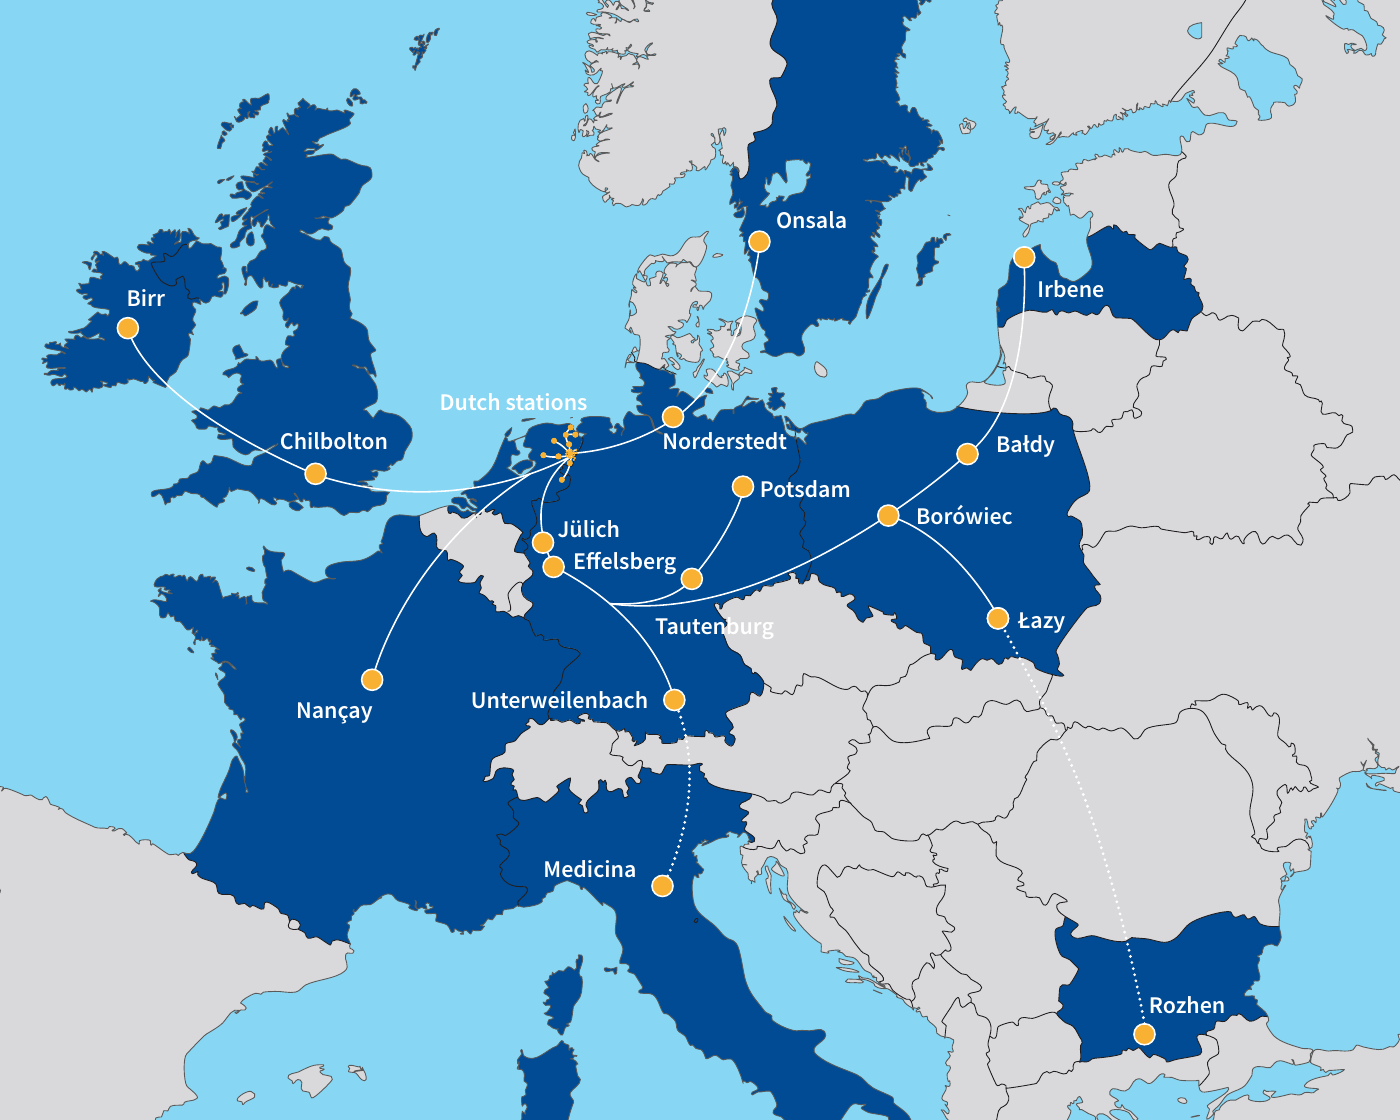
\includegraphics[width=0.9\linewidth]{img/lofar-map.png}
  \end{minipage}\hfill
  \begin{minipage}[t]{0.568\linewidth}
    \centering
    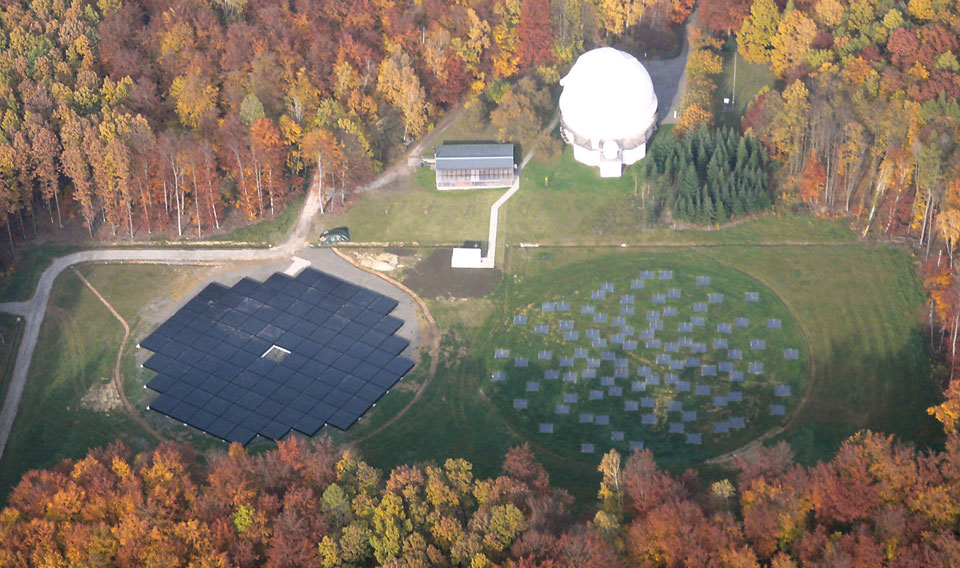
\includegraphics[width=0.9\linewidth]{img/LOFAR-station-Tautenburg1-Germany-Copyright-Michael-Pluto.png}
  \end{minipage}
  \caption[LOFAR station network and Tautenburg station]{The Dutch and international LOFAR station network map (left; map credit: ASTRON) and the LOFAR station at Tautenburg, Germany (right; photograph by Michael Pluto).}
  \label{fig:lofar_network}
\end{figure}

The LOFAR Two-metre Sky Survey (LoTSS) is the principal northern-hemisphere extragalactic survey conducted with this instrument. LoTSS observes with the High-Band Antenna from $120$ to $168\,\mathrm{MHz}$, with a central frequency of $144\,\mathrm{MHz}$. Its second data release, LoTSS-DR2, covers $5{,}634\,\mathrm{deg}^{2}$ in two contiguous regions of the northern sky at an angular resolution of $6''$, with a median rms noise of $83\,\mu\mathrm{Jy\,beam^{-1}}$, and yields a total catalogue of $4{,}396{,}228$ radio sources \citep{Shimwell2022}. At this resolution, a source with $\mathrm{LAS}=60''$ spans approximately ten synthesised beam widths, permitting resolved morphological information to be recovered, although the visibility of individual cores, lobes, hotspots, and bent tails also depends on their surface brightness and structure.

For radio-galaxy studies, catalogue components must be associated into physical radio sources and linked, where possible, to optical or infrared host galaxies. For LoTSS-DR2, these associations are provided by a value-added catalogue combining likelihood-ratio cross-matching against optical and infrared imaging, the citizen-science project Radio Galaxy Zoo: LOFAR, and direct visual inspection by domain experts \citep{Hardcastle2023}. Within the area covered by suitable optical imaging, the catalogue assigns an optical or infrared identification to $85\,\%$ of LoTSS-DR2 sources and a spectroscopic or photometric redshift to $58\,\%$. It also supplies source associations and size information needed to construct a catalogue of resolved radio galaxies.

The third data release, LoTSS-DR3, substantially extends this coverage: it contains $12{,}950\,\mathrm{h}$ of observations over $19{,}035\,\mathrm{deg}^{2}$, corresponding to $88\,\%$ of the northern sky, and catalogues $13{,}667{,}877$ radio sources at $6''$ resolution, increasing to $9''$ below declination $10^{\circ}$ \citep{Shimwell2026}. A dedicated catalogue of galaxy clusters with diffuse radio emission has also been compiled from the DR3 imaging \citep{Stuardi2026}. The catalogue-scale sample in this thesis remains based on DR2 because it was selected using the host associations and angular-size information in the DR2 value-added catalogue. We describe the precise data products and selection criteria in Chapter~\ref{sec:data}.

\subsection{Radio galaxies and the morphological taxonomy}
\label{sec:bg_taxonomy}

Radio galaxies are radio-loud active galactic nuclei whose central engines launch collimated plasma jets from the vicinity of an accreting supermassive black hole.
Synchrotron emission traces a compact radio core, the jets, and the lobes or plumes inflated where the jets deposit energy into the surrounding medium. 
Shocks near the ends of powerful jets can produce compact hotspots. Hence, the observed morphology encodes both the transport of energy by the jets and
their interaction with the gaseous environment across galactic and cluster scales \citep{HardcastleCroston2020}.
The most widely used morphological division is the Fanaroff--Riley (FR) classification. 
\citet{Fanaroff1974} defined the ratio $R_{\mathrm{FR}}$ of the separation of the highest-surface-brightness regions on opposite sides of the host, excluding the compact central core, to the total source extent.
FR\,I sources have $R_{\mathrm{FR}}<0.5$ and are centre-brightened, whereas FR\,II sources have $R_{\mathrm{FR}}>0.5$ and are edge-brightened (top-left and top-middle sources in Fig.~\ref{fig:radio_morphology_overview}). 
In the original 3CR sample, the transition occurred near a 178-MHz radio power of $P_{178}\simeq2\times10^{25}\,\mathrm{W\,Hz^{-1}\,sr^{-1}}$ under the cosmology adopted in that work. This was an empirical correlation, not a strict physical boundary. Lower-power jets are typically more susceptible to disruption and deceleration into diffuse plumes, whereas more powerful jets can remain collimated until they terminate in hotspots. Nevertheless, jet power, host-galaxy properties, and environment all influence the resulting morphology \citep{HardcastleCroston2020}.

Clearly, the radio-galaxy population is not exhausted by this binary scheme. FR\,0 sources are compact, core-dominated radio galaxies with weak or absent extended emission \citep{Baldi2015}. 
Bent-tail sources are distinguished mostly by geometry rather than by a unique formation mechanism.
Narrow-angle-tail (NAT) sources have closely swept-back jets or tails and are commonly associated with ram pressure produced by relative motion between the galaxy and the intracluster medium (ICM) (top-right source in Fig.~\ref{fig:radio_morphology_overview}).
Wide-angle-tail (WAT) sources have a broader opening angle, often with initially collimated jets that flare into bent plumes around a cluster-dominant galaxy (bottom-left in Fig.~\ref{fig:radio_morphology_overview}). Relative galaxy--ICM motion associated with cluster mergers can contribute to their bending \citep{Sakelliou2000}.
Head-tail (HT) is a broader descriptive label for emission trailing away from a bright head and does not require a single resolved tail (bottom-middle in Fig.~\ref{fig:radio_morphology_overview}). These forms encode interactions between the radio jets, the motion of the host, and the surrounding gas.
Relaxed double (RD) sources are symmetric relaxed structures, with no visible jets and less interaction with a dense environment (bottom-right in Fig.~\ref{fig:radio_morphology_overview}). The absence of compact cores, hotspots and jets suggests that these RDs represent the late evolutionary stage of radio galaxies \citep{Chilufya2025}.

\begin{figure}[ht]
  \centering
  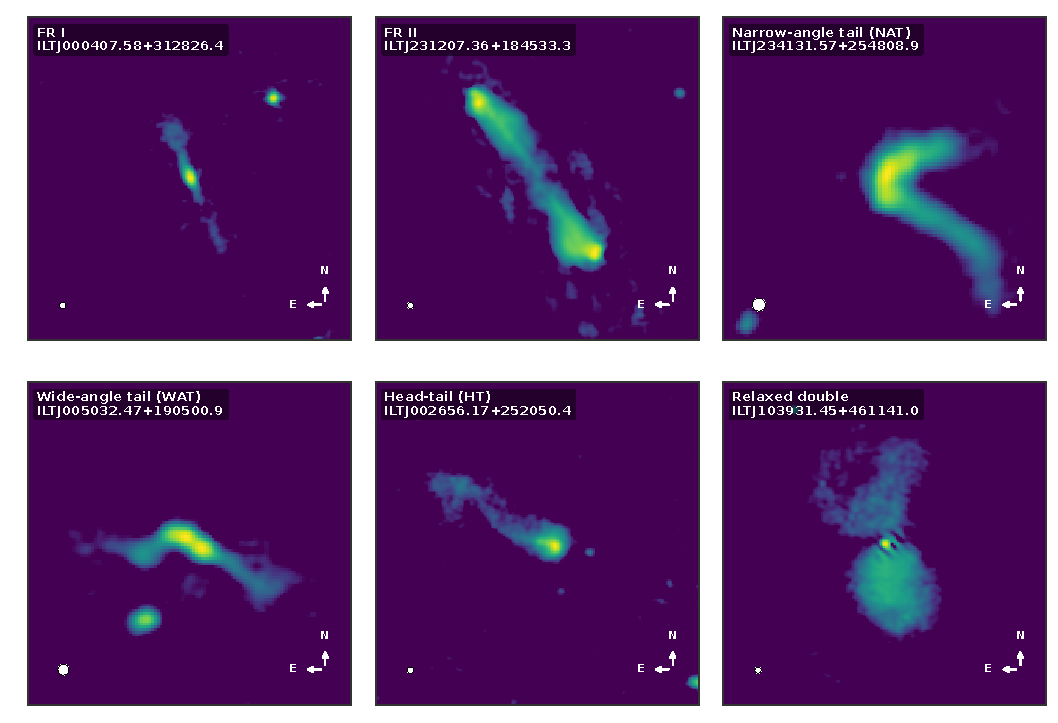
\includegraphics[width=0.9\textwidth]{img/radio_morphology_overview.pdf}
  \caption[Examples of radio-galaxy morphologies]{Representative host-centred LoTSS-DR2 144-MHz images of the radio-galaxy morphologies classified by \citet{Chilufya2025}. Each field spans $1.5\times\mathrm{LAS}$; the synthesised beam is shown at lower left, with north up and east left.}
  \label{fig:radio_morphology_overview}
\end{figure}

LoTSS has demonstrated that these morphological categories overlap strongly in their physical properties. Using $5{,}805$ extended radio-loud AGN from LoTSS-DR1, \citet{Mingo2019} found significant overlap between the FR\,I and FR\,II luminosity distributions and a population of FR\,IIs extending three orders of magnitude below the canonical FR break at $L_{150}\sim10^{26}\,\mathrm{W\,Hz^{-1}}$.
In LoTSS-DR2, \citet{Clews2025} classified $3{,}590$ FR\,IIs and $2{,}354$ FR\,Is at $z\leq0.8$. 
Near the FR divide, FR\,I morphology is more frequent in more massive hosts, but no robust correlation between the break luminosity and stellar mass remains after selection effects are considered. This dependence on multiple source and host properties reinforces that FR morphology is not determined by a single luminosity division.
\citet{Chilufya2025} studied $2{,}828$ extended radio-loud AGN with $\mathrm{LAS}>60''$ and found that almost all FR\,Is in their spectroscopic sample are low-excitation radio galaxies, whereas high-excitation objects occur predominantly among luminous FR\,IIs; nevertheless, no single radio or host property fully determines accretion mode. 
Finally, \citet{Horton2025} catalogued $9{,}985$ large, bright LoTSS-DR2 sources using broad morphologies and finer structural attributes, finding at least one possible jet-precession indicator in $28\,\%$ of the sample. 
Together, these results motivate a morphology taxonomy richer than a strict FR dichotomy.

Radio galaxies can also be distinguished by their physical scale and activity history.
For instance, giant radio galaxies have projected sizes above approximately $0.7\,\mathrm{Mpc}$; \citet{Dabhade2020} identified $239$ in LoTSS-DR1, including seven larger than $2\,\mathrm{Mpc}$.
Remnant and restarted radio galaxies instead preserve diffuse plasma from earlier episodes of jet activity, sometimes alongside newly formed jets or lobes. 
These properties can coexist with the FR and bent-tail labels and further broaden the range of radio-galaxy appearances.

Large morphology catalogues also differ in how their labels are constructed. \citet{Clews2025} used a semi-automated method based on radio-source ridgelines, whereas \citet{Horton2025} assigned detailed, multi-attribute labels through visual inspection of LoTSS images. \citet{Chilufya2025} used visual classification supported by higher-resolution VLASS observations and multiple independent classifiers. 
Differences in source selection, available image information, and classification specificity mean that these catalogues provide distinct reference schemes instead of establishing ground-truth labels.

\subsection{Diffuse radio emission in galaxy clusters}
\label{sec:bg_diffuse}

Galaxy clusters contain a hot, magnetised intracluster medium (ICM) in which relativistic electrons produce extended synchrotron emission.
This diffuse emission is not associated one-to-one with an optical galaxy and is conventionally divided into radio haloes, mini-haloes, and radio relics \citep{vanWeeren2019} (Figure~\ref{fig:cluster_diffuse_classes}).
These categories describe different locations and morphologies within a galaxy cluster. 
Interestingly, they do not imply that active galaxies are irrelevant to this emission: fossil plasma deposited by earlier AGN activity may provide seed particles that are subsequently re-energised in the ICM.

\begin{figure}[H]
  \centering
  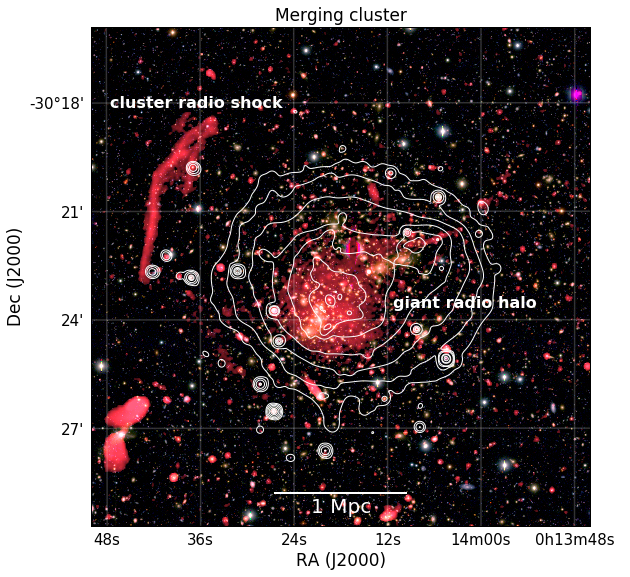
\includegraphics[width=0.45\textwidth]{img/a2744_halo_relic.png}\hfill
  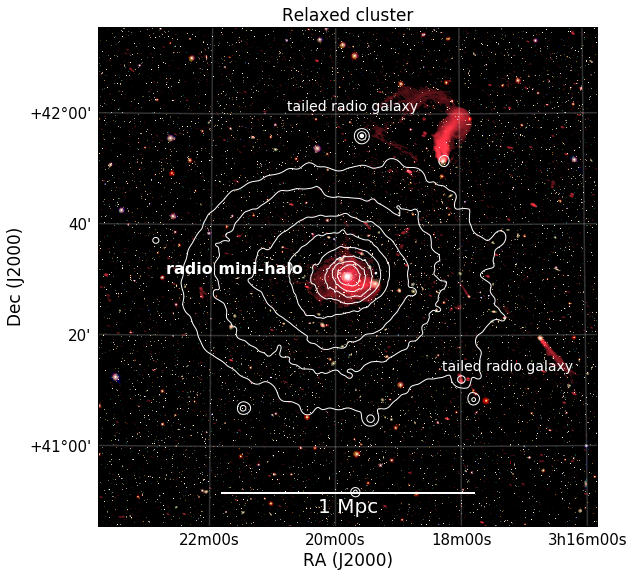
\includegraphics[width=0.45\textwidth]{img/perseus_minihalo.png}
  \caption[Examples of radio haloes, relics and mini-haloes]{Radio halo and relic emission in Abell~2744 (left) and the Perseus mini-halo (right). Reproduced from \citet{vanWeeren2019} under CC BY~4.0.}
  \label{fig:cluster_diffuse_classes}
\end{figure}

Radio relics are often elongated, arc-like sources found mainly in the periphery of merging clusters and are frequently polarised at gigahertz frequencies.
Their locations and spectral properties associate them with merger-driven shock waves, where electrons may be freshly accelerated or re-accelerated from a fossil population. Revived fossil or phoenix plasma is a related but distinct diffuse-emission category; here, relic refers to the selected elongated cluster sources \citep{vanWeeren2019}.
The northern ``Sausage'' relic in CIZA\,J$2242.8{+}5301$ is a well-studied example (Fig.~\ref{fig:sausage_relic}). It forms a thin, nearly $2\,\mathrm{Mpc}$ arc with aligned magnetic fields and a radio spectrum that steepens downstream from the outer edge \citep{vanWeeren2010}.

Radio haloes instead occupy the central regions of merging clusters, extend over scales of order a megaparsec, and broadly follow the distribution of the thermal ICM.
Turbulent re-acceleration following a merger is a leading explanation for their distributed emission.
Mini-haloes are smaller, typically spanning about $100$--$500\,\mathrm{kpc}$ around the brightest cluster galaxy in relaxed cool-core clusters.
\begin{wrapfigure}{r}{0.45\textwidth}
\vspace{-0.5cm}
  \centering
  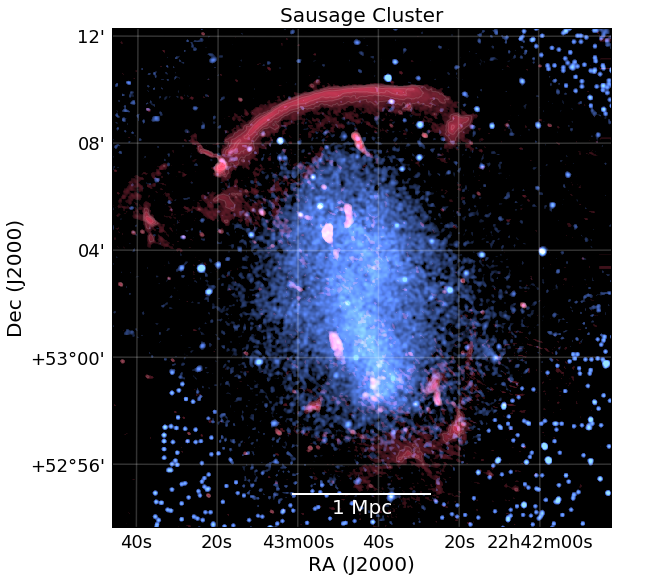
\includegraphics[width=\linewidth]{img/sausage_relic.png}
  \caption[Radio and X-ray emission in the Sausage cluster]{The Sausage cluster: 610-MHz radio (red) and X-ray (blue) emission. Reproduced from \citet{vanWeeren2019} under CC BY~4.0.}
  \label{fig:sausage_relic}
\vspace{-1cm}
\end{wrapfigure}
Sloshing-induced turbulence and re-acceleration of seed particles supplied by the central radio galaxy are among the proposed mechanisms.
Haloes and mini-haloes can contain substantial substructure, but unlike relics their emission is not localised to an identifiable peripheral shock \citep{vanWeeren2019}.

Radio relics have a different physical origin from radio galaxies, yet their diffuse structures may resemble parts of radio-galaxy emission. 
This motivates examining whether a model trained to distinguish radio-galaxy morphologies assigns similar descriptions to relics. We explore this question using selected, manually masked relic images described in Section~\ref{sec:data_relics}. Nevertheless, this test does not establish whether the model can recognise unfamiliar sources in general.

\subsection{Self-supervised representations and clustering}
\label{sec:bg_ssl}

Machine learning (ML) uses models fitted to data to recognise patterns and make predictions. In astronomy, it provides tools for analysing large survey datasets whose scale and diversity make detailed manual inspection difficult.
Deep learning is a subset of ML in which neural networks with multiple processing layers organised within a particular architecture learn successive representations of the input. For image inputs, these representations can capture spatial structure directly from pixel intensities. Applications in radio astronomy include source detection, morphological classification, and searches for similar or unusual objects~\citep{Slijepcevic2024,Riggi2024}. However, the available images greatly outnumber those with reliable expert labels, motivating methods that can learn useful representations from unlabelled observations~\citep{Slijepcevic2024}.

Supervised learning trains a model from images paired with class labels, and unsupervised learning searches for structure without such labels.
Self-supervised learning also uses unlabelled data, but constructs a training objective from the data themselves.
In this thesis, self-supervised pre-training first teaches a network to encode radio-source structure.
The pre-trained network is then fine-tuned on a smaller labelled sample for morphological classification~\citep{Nicolas2025}.

An encoder $f_\theta$ maps an input image $x$ to a finite-dimensional representation $h=f_\theta(x)$, also called an embedding. 
Distances in the embedding space express which image features the encoder regards as similar.
A morphology-aware embedding should place structurally similar radio sources close together even when their orientation or brightness differs.
Subsequently, this representation space can be clustered to construct morphological groups and used as the input to a classifier~\citep{Nicolas2025,Slijepcevic2024}.

The framework adopted by \citet{Nicolas2025} and followed here is \textit{A Simple Framework for Contrastive Learning of Visual Representations} \citep[SimCLR;][]{Chen2020}.
Two independently augmented views of each image form a positive pair.
Views originating from other images in the same minibatch act as negative examples.
These comparisons provide a supervisory signal without requiring morphology labels.
The augmentations are assumed to preserve the underlying source morphology while changing nuisance properties such as orientation or brightness. Bringing the resulting positive views together therefore teaches the encoder invariance to those transformations. A minibatch is the group of images processed together in one optimisation step.
An encoder $f_\theta$ and a projection head $g_\phi$ are trained jointly so that projected positive-pair embeddings are similar and negative-pair embeddings are separated. 
For $2N$ views generated from $N$ images, the contribution of a positive pair $(i,j)$ to the normalised temperature-scaled cross-entropy (NT-Xent) loss is
\begin{equation}
\mathcal{L}_{i,j} = -\log \frac{\exp\!\left(\mathrm{sim}(z_i,z_j)/\tau\right)}{\sum_{k=1}^{2N}\mathbf{1}_{[k\neq i]}\,\exp\!\left(\mathrm{sim}(z_i,z_k)/\tau\right)},
\label{eq:ntxent}
\end{equation}
where $z=g_\phi(f_\theta(x))$, $\mathrm{sim}(u,v)=u\cdot v/(\lVert u\rVert\lVert v\rVert)$ is cosine similarity, and $\tau$ controls how strongly the loss distinguishes similar from dissimilar embeddings.
The indicator excludes the anchor from the denominator. After pre-training, the projection head is discarded and the encoder is retained for downstream use.

For an anchor view \(i\), the numerator measures its similarity to the corresponding positive view \(j\). The denominator compares that positive similarity with the similarities between \(i\) and every other view in the minibatch, excluding only \(i\) itself. Minimising the loss therefore increases the positive pair's similarity relative to the competing views. The temperature \(\tau\) controls how strongly differences between similarities are emphasised; each of the two views is used in turn as the anchor, and the resulting contributions are averaged.

Standard SimCLR has a limitation for radio-morphology applications: views originating from other images in the minibatch are treated as negative examples.
Distinct sources with nearly identical morphology may therefore be pushed apart in the representation space.
The random structural view (RSV) introduced by \citet{Nicolas2025} addresses this limitation by allowing one augmented view to be replaced by a view of a structurally similar source identified using semi-invariant structural similarity.
Thus, positive pairs can connect distinct sources with similar morphology, encouraging the representation space to encode cross-source structural similarity.
The transformations and selection parameters used in this thesis are specified in Sec.~\ref{sec:method_simclr}.

After pre-training, the learned representations must be organised into candidate morphological groups.
Principal component analysis (PCA) projects the high-dimensional representations onto orthogonal axes ordered by the variance they explain \citep{Jolliffe2016}.
This linear construction is mathematically transparent: every principal component is a linear combination of the encoder features, its contribution is quantified by its explained variance, and the reduced dimensionality can be selected through an explicit retained-variance criterion.
Hierarchical density-based spatial clustering of applications with noise (HDBSCAN) is applied here to the retained multidimensional PCA representation.
Unlike methods that require a predetermined number of approximately spherical clusters, HDBSCAN identifies dense regions with potentially different shapes and densities and can leave isolated sources unassigned as noise \citep{Campello2013,McInnes2017}.
These properties are useful for an uncurated radio-source sample containing rare morphologies, artefacts, and ambiguous sources. 
For visualisation, the first three principal components can be plotted and coloured by the HDBSCAN assignments. 
Visual inspection of the source images within each resulting cluster then assesses morphological coherence and supports consolidation into a labelled subsample. 
The adopted PCA and HDBSCAN configuration is specified in Sec.~\ref{sec:method_simclr}.

\subsection{Deep ensembles and predictive uncertainty}
\label{sec:bg_ensembles}

The output probabilities of a single neural network by themselves can be overconfident. They do not quantify epistemic uncertainty due to training data limitations or model choice.
To increase the reliability of the probability estimates for the class predictions, \citet{Nicolas2025} adopted a deep ensemble.
\citet{Lakshminarayanan2017} proposed that training an ensemble of randomly initialised networks ($M$ classifiers with the same architecture) can yield better-calibrated probabilities and stronger out-of-distribution detection, while training and inference costs scale approximately with ensemble size.

Let $\mathbf{p}_m(x)=(p_m^c(x))_{c\in\mathcal{K}}$ denote the class-probability vector predicted for source image $x$ by ensemble member $m \in \{1,\ldots,M\}$, where $\mathcal{K}$ is the class set with cardinality $K=|\mathcal{K}|$. The ensemble mean vector $\bar{\mathbf{p}}(x)$ and ensemble agreement are defined as
\begin{equation}
\bar p^{\,c}(x) \;=\; \frac{1}{M}\sum_{m=1}^{M} p_m^c(x), \qquad
A(x) \;=\; \frac{1}{M}\sum_{m=1}^{M} \mathbf{1}\!\left[\arg\max_{c\in\mathcal{K}} p_m^c(x) = \hat{y}\right],
\label{eq:ensmean}
\end{equation}
where $A(x)\in[0,1]$ measures the fraction of ensemble members whose top-predicted class coincides with the ensemble-mean decision $\hat{y} = \arg\max_{c\in\mathcal{K}} \bar p^{\,c}(x)$. The total predictive uncertainty of the ensemble is captured by the entropy of the mean distribution,
\begin{equation}
H[\bar{\mathbf{p}}](x) \;=\; -\sum_{c\in\mathcal{K}} \bar p^{\,c}(x)\,\log \bar p^{\,c}(x),
\label{eq:H}
\end{equation}
which is maximised at $\log K$ for a uniform distribution over the $K$ classes.

\begin{table}[H]
  \centering
  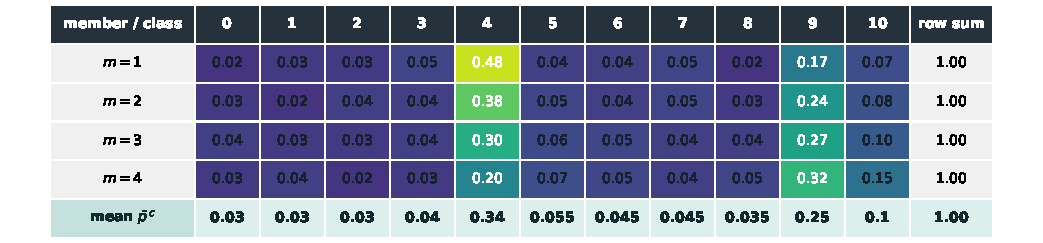
\includegraphics[width=\linewidth]{img/srg_component_walkthrough.pdf}
  \caption[Example ensemble probabilities and agreement]{Illustrative class-probability vectors for four ensemble members and their component-wise mean. Each member's predicted class is the class with the largest probability in its row, whereas the ensemble decision $\hat{y}$ is the class with the largest mean probability. Here, $\hat{y}=4$ and three of the four members also predict class~4, giving $A=3/4$. Each row sums to one.}
  \label{tab:ensemble_probability_components}
\end{table}

The total uncertainty $H[\bar{\mathbf{p}}]$ can be decomposed algebraically into terms commonly associated with the data (aleatoric) and model (epistemic) components. The model-disagreement term, commonly interpreted as epistemic uncertainty, is the mutual information ($\mathrm{MI}$) between the class prediction and the ensemble index $m$ when members are treated as uniformly sampled models. It can be expressed in closed form as the difference between the entropy of the mean and the mean of the per-member entropies \citep{Houlsby2011,Depeweg2018},
\begin{equation}
\mathrm{MI}(x) \;=\; H[\bar{\mathbf{p}}](x) \;-\; \frac{1}{M}\sum_{m=1}^{M} H[\mathbf{p}_m](x).
\label{eq:MI}
\end{equation}

All ensemble members start from the same pre-trained encoder weights and biases, which are subsequently updated during fine-tuning. The resulting independently fine-tuned members are not exact samples from a posterior distribution. Therefore, $\mathrm{MI}(x)$ is interpreted here as an empirical measure of model disagreement, not as an exact Bayesian separation of aleatoric and epistemic uncertainty.

The mutual information is bounded above by $\log K$, as is $H$. Compared to the agreement rate $A$, $\mathrm{MI}$ captures disagreement between ensemble members across the full predicted distribution.
It can therefore respond to differences that leave the top class unchanged, but it is not universally more sensitive than $A$.
Henceforth, the quantities $(A,H,\mathrm{MI})$ are used as complementary uncertainty-related inputs to define the reliability factor $R(x)$ (see Sec.~\ref{sec:method_srg}).
